\chapter{Development of the switching model}
\label{chp:switching_model}

\graphicspath{{images/development_of_switching_model/}}

\section{The switching model}

As illustrated in chapter~\ref{chp:background}, the Braginskii model of viscosity fails to capture the transition between isotropic and anisotropic viscosity in the vicinity of magnetic null points. Computational solutions such as refining the mesh near the null or implementing a multigrid method may help to improve the resolution and better resolve the viscosity transition region, however approaches like these can be complex to implement in existing codes. A simpler way to improve the resolution is to artificially scale $|\vec{B}|$ in the expression for the parallel Braginskii transport parameter~\ref{eq:perp_visc_coeff} in order to enlarge the isotropic region to resolvable scales. The scaling factor applied to $|\vec{B}|$ effectively controls the interpolation between isotropic and parallel tensors. Going a step further and considering more general forms of interpolation, we can construct a variety of viscosity models useful in different circumstances and incorporating different physics.

The switching model is a model of viscosity that approximates the full Braginskii tensor throughout most of the solar corona. In strong magnetic fields, the Braginskii tensor can be approximated by the purely parallel term while in weak or null fields, the tensor reduces to that of fully isotropic, Newtonian viscosity. Between these extremes the perpendicular and drift components of the tensor can become relevant~\cite{erdelyiResonantAbsorptionAlfven1995a}. However, at the resolutions typically studied in 3D MHD simulations (between $300$ and $1000$ grid points per dimension) null points are likely to be poorly resolved. This is particularly true in simulations where null points are not the main focus of the simulation, but are dynamically created by some process. By stripping out the perpendicular and drift elements of the full Braginskii tensor, the switching model presents a cleaner, better-resolved viscous model by focusing on what are, in many cases, the most physically important parts of anisotropic viscosity in the solar corona: the parallel and isotropic components. The idea at the core of the model is the interpolation between the parallel and isotropic tensors, mirroring the way in which the Braginskii tensor changes in strong and weak fields.

\subsection{The von Mises switching function}

The switching model takes the form of an interpolation between the isotropic and parallel tensors,
\begin{equation}
  \label{eq:switching_model_simple}
\ten{\sigma}_{\text{swi}} = \eta_0 \left( 1 - s^2 \right) \ten{W} + \eta_0 s^2 \ten{W}^{(0)},
\end{equation}
or
\begin{equation}
  \label{eq:switching_model}
\ten{\sigma}_{\text{swi}} = \eta_0 \left( 1 - s^2 \right) \ten{W} + \eta_0 s^2 \left[\frac{3}{2}(\ten{W}\vec{b}\cdot\vec{b}) \left( \vec{b} \otimes \vec{b} - \frac{1}{3}\ten{I} \right)\right],
\end{equation}
where the interpolation is governed by the square of the interpolation function, $s(|\vec{B}|)^2$. This takes the form,
\begin{equation}
  \label{eq:switching_function}
s(|\vec{B}|) = \frac{3 \exp[2a]}{2\sqrt{2\pi a} \text{erfi}[\sqrt{2a}]} - \frac{1}{2}\left[ 1 + \frac{3}{4a} \right],
\end{equation}
where $a(|\vec{B}|)$ is a constitutive function which controls the sensitivity of the interpolation function to a change in magnetic field strength. Throughout this thesis, the choice $a(|\vec{B}|) = a_0 |\vec{B}|^2$ is made, where $a_0$ is a parameter which effectively controls the size of the isotropic region near magnetic null points. Other choices are discussed later in this chapter. Note also the use of erfi, the imaginary error function.

\subsection{Derivation of the von Mises switching function}

The switching function is derived during the derivation of the structure tensor $\ten{H}$, a tensor which encodes the anisotropy of the momentum transport. The following derivation of $\ten{H}$ is related to that of~\cite{gasserHyperelasticModellingArterial2006} who use a similar method to derive a structure tensor to model the orientations of collagen fibres in arterial walls. The structure tensor can be used to write a general form for viscous stress tensors which is then used to construct the switching model as a variation on the Braginskii stress tensor.

For the purposes of this derivation, we assume the magnetic field is non-zero, allowing us to use the unit vector $\vec{b} = \vec{B}/|\vec{B}|$. Importantly, this direction is known to give the preferred orientation of momentum transport~\cite{braginskiiTransportProcessesPlasma1965}.

We consider a probability density function $f_{\vec{x}} : \mathbb{S}^2 \to \mathbb{R}^+$ defined over the unit sphere $\mathbb{S}^2$, where $f_\vec{x}(\vec{t}) \text{d}\omega$ gives the probability of the momentum transport through the position $\vec{x}$ orienting along $\vec{t}$ within the solid angle d$\omega$. Since this is a probability density function, it must satisfy the normalisation condition,
\begin{equation}
  \label{eq:normalisation_condition}
  \frac{1}{4\pi} \int_{\mathbb{s}^2} f_\vec{x}(\vec{t})\ \text{d}\omega = 1.
\end{equation}

Single-fluid MHD does not typically rely on the specific orientation of the local magnetic field, only the direction, that is, it is invariant under the transformation $\vec{b} \to -\vec{b}$. Since this is a model of viscosity intended for use in single-fluid MHD, we assume the direction of momentum transport is similarly invariant. This gives $f_\vec{x}(\vec{t} = f_\vec{x}(-\vec{t}$ and the first moment of the distribution is zero as a result. The second moment is the variance tensor, written
\begin{equation}
  \label{eq:variance_tensor}
\ten{M} = \frac{1}{4\pi} \int_{\mathbb{s}^2} f_\vec{x}(\vec{t} \otimes \vec{t}) \ \text{d}\omega.
\end{equation}
Using an orthonormal basis ${\vec{e}_1, \vec{e}_2, \vec{e}_3}$, $\ten{M}$ can be rewritten as
\begin{equation}
  \label{eq:variance_tensor_basis}
  \ten{M} = \sum_{i,j=1}^{3} \alpha_{ij} \vec{e}_i \otimes \vec{e}_j,
\end{equation}
where
\begin{equation}
  \label{eq:variance_components}
\alpha_{ij} = \frac{1}{4\pi} \int_{\mathbb{s}^2} f_\vec{x}(\vec{t} t_i t_j \text{d}\omega,
\end{equation}
with $t_i$ being the components of $\vec{t}$ in our chosen basis.

Without loss of generality, we consider a basis where the magnetic field is aligned with $\vec{e}_3$, that is $\vec{e}_3 = \vec{b}$. We may then characterise $\vec{t}$ in terms of two Euler angles, $\theta \in [0, \pi]$ and $\phi \in [0, 2\pi)$,
\begin{equation}
  \label{eq:t_in_euler}
\vec{t} = \sin \theta \cos \phi \vec{e}_1 + \sin \theta \sin \phi \vec{e}_2 + \cos \theta \vec{e}_3.
\end{equation}
By rotational symmetry around $\vec{e}_3$, the density function must be independent of $\phi$, hence the normalisation condition becomes
\begin{equation}
  \label{eq:normalisation_condition2}
\frac{1}{2} \int_0^{\pi} f_{\vec{x}} (\theta) \sin \theta\ \text{d} \theta = 1,
\end{equation}
and the variance tensor reduces to a diagonal tensor with components
\begin{equation}
  \label{eq:variance_diagonals}
\alpha_{11} = \alpha_{22} = \kappa, \quad \alpha_{33} = 1-2\kappa,
\end{equation}
where $\kappa$ is a parameter called the dispersion parameter which measures the anisotropy of the momentum transport. This is written
\begin{equation}
  \label{eq:kappa}
\kappa = \frac{1}{4} \int_0^{\pi} f_{\vec{x}} (\theta) \sin^3 \theta\ \text{d} \theta.
\end{equation}
The full variance tensor can then be written in any basis as
\begin{equation}
  \label{eq:variance_tensor_compact}
\ten{M} = \kappa \ten{I} + (1-3\kappa) \vec{b} \otimes \vec{b},
\end{equation}
and the structure tensor $\ten{H}$, the traceless part of $\ten{M}$, is written
\begin{equation}
  \label{eq:structure_tensor}
\ten{H} = \ten{M} - \tfrac{1}{3} \ten{I} = s \left ( \vec{b} \otimes \vec{b} - \tfrac{1}{3} \ten{I} \right), \quad s = 1 - 3\kappa,
\end{equation}
where we now properly introduce the interpolation function $s$, first stated in equation~\ref{eq:switching_function}.

\begin{figure}[t]
  \centering
  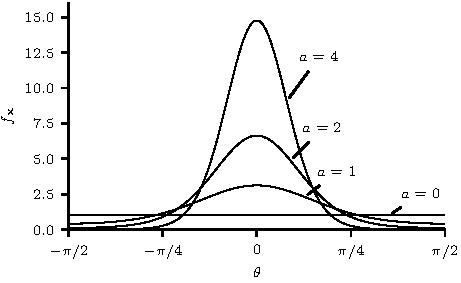
\includegraphics[width=0.5\linewidth]{von_mises_distribution.pdf}
  \caption{von Mises distribution for different values of the concentration parameter $a$.}%
  \label{fig:von_mises_distribution}
\end{figure}

The preceding derivation has been performed using a general orientation density function $f_\vec{x}(\vec{t})$, however in order to proceed further, we much choose a specific form for the distribution. A natural choice is the transversely isotropic and $\pi$-periodic von Mises distribution which essentially maps the normal distribution onto the unit sphere. Modifying the distribution to satisfy the normalisation condition~\ref{eq:normalisation_condition2}, it is written
\begin{equation}
  \label{eq:von_mises}
f_{\vec{x}}(\theta) = 2 \sqrt{\frac{2a}{\pi}} \frac{\exp(2a \cos^2 \theta)}{\text{erfi}(\sqrt{2a})},
\end{equation}
where erfi$(x) = -i$erf$(ix)$ is the imaginary error function and $a$ is a positive quantity called the concentration parameter which controls the shape of the distribution, as illustrated in figure~\ref{fig:von_mises_distribution}. As $a \to 0$, $f_{\vec{x}} \to 1$, modelling isotropic momentum transport, while as $a \to + \infty$, $f_{\vec{X}}$ tends to the Dirac delta function, modelling strong-field, parallel momentum transport. Hence, this distribution models the asymptotic behaviour we desire.

\begin{figure}[t]
  \centering
  \includegraphics[width=0.5\linewidth]{s_against_a.pdf}
  \caption{Plots of $s$, $s^2$ as functions of $a$ including the asymptotic limit as $a \to 0$.}%
  \label{fig:s_against_a}
\end{figure}

Inserting~\ref{eq:von_mises} into~\ref{eq:kappa} and integrating gives the analytical expression
\begin{equation}
  \label{eq:kappa_analytical}
\kappa = \frac{1}{2} \left( 1 + \frac{1}{4a} \right) - \frac{\exp(2a)}{2 \sqrt{2 \pi a } \text{erfi} ( \sqrt{2 a} )},
\end{equation}
which allows us to write $s(a)$ as 
\begin{equation}
  \label{eq:switching_function_a}
s(a) = \frac{3 \exp[2a]}{2\sqrt{2\pi a} \text{erfi}[\sqrt{2a}]} - \frac{1}{2}\left[ 1 + \frac{3}{4a} \right].
\end{equation}
Note that asymptotically,
\begin{equation}
  \label{eq:asymptotic_s}
s \sim \tfrac{4}{15} a + \mathcal{O}(a^2) \quad \text{as} \ a \to 0,
\end{equation}
and $s to 1$ as $a \to +\infty$. The switching function $s$ and the asymptotic limit as $a \to 0$ are shown in figure~\ref{fig:s_against_a}.

We now must link the magnetic field strength to the concentration parameter so that $s$ has the correct properties. We assume $a$ is a function of $|\vec{B}|$,
\begin{equation}
  a = \hat{a}(|\vec{B}|).
\end{equation}
Since
\begin{enumerate}[label={(\arabic*)}]
  \item the probability that momentum transport orients along the magnetic field increases as $|\vec{B}|$ increases,
  \item the momentum transport aligns perfectly with the magnetic field when $|\vec{B}|$ is large enough,
  \item the momentum transport has no preferred direction when $|\vec{B}|$ is small,
\end{enumerate}
we require $\hat{a}$ to satisfy the following properties:
\begin{enumerate}[label={(\roman*)}]
  \item $\hat{a}$ is a non-negative, increasing function of $|\vec{B}|$,
  \item $\hat{a}(|\vec{B}|) \to + \infty$ as $|\vec{B}| \to + \infty$,
  \item lim$_{\vec{B} to \vec{0}}(\hat{a}(|\vec{B}|)/ |\vec{B}|^2) \in \mathbb{R}$.
\end{enumerate}
Property (iii) requires $\hat{a} \sim \mathcal{O}(|\vec{B}|^n)$ where $n \geq 2$ in the asymptotic limit $|\vec{B}| \to 0$. The reason for this requirement will be clear in a few lines as we remove the assumption that $|\vec{B}| \neq 0$.

Rewriting $\ten{H}$ without the use of the unit vector $\vec{b}$ gives
\begin{equation}
  \label{eq:structure_tensor2}
  \ten{H} = \frac{s(|\vec{B}|)}{|\vec{B}|^2}\left( \vec{B} \otimes \vec{B} - \frac{|\vec{B}|^2}{3}\ten{I} \right),
\end{equation}
where $s$ is now a function of $|\vec{B}|$. For $\ten{H}$ to remain finite as $|\vec{B}| \to 0$, $s \sim \mathcal{O}(|\vec{B}|^n)$ where $n \geq 2$ in the asymptotic limit $|\vec{B}| \to 0$ which is satisfied because of property (iii) and~\ref{eq:asymptotic_s}. This allows the structure tensor to be utilised in any magnetic topology, including those involving magnetic null points. The simplest non-trivial form for the concentration parameter is $a = a_0 |\vec{B}|^2$ for some constant $a_0 > 0$.

It can be shown (see~\cite{mactaggartBraginskiiMagnetohydrodynamicsArbitrary2017}) that the most general form for a viscous stress tensor is
\begin{equation}
  \label{eq:general_viscous_stress_tensor}
\sigma_V = \beta_1 \ten{W} + \beta_2 [ \ten{W}^2 - \tfrac{1}{3} (\ten{W}^2)\ten{I}]\\
+ \beta_3 \ten{H} + \beta_4 [ \ten{W} \ten{H} + \ten{H} \ten{W} - \tfrac{2}{3} ( \ten{W} \ten{H}) \ten{I}]\\
+ \beta_5 [ \ten{W}^2 \ten{H} + \ten{H} \ten{W}^2 - \tfrac{2}{3} ( \ten{W}^2 \ten{H} ) \ten{I}.
\end{equation}
Isotropic viscosity can be trivially recovered by setting $\beta_1 = \eta_0$ and all other $\beta$ to zero. The Braginskii tensor~\ref{eq:braginskii_tensor} can be written in this form by taking
\begin{equation}
  \label{eq:brag_betas}
\beta_1 = \frac{2 \eta_2 + \eta_1}{3},\\
\beta_3 = \frac{3 \eta_0 + \eta_1 - 4\eta_2}{s^2}  (\ten{D}\ten{H}),\\
\beta_4 = \frac{\eta_2 - \eta_1}{s},
\end{equation}
with the remaining values of $\beta$ being zero. We can construct a variation on the Braginskii tensor by taking
\begin{equation}
  \label{eq:switching_betas}
\beta_1 = \eta_0 [1 - s^2],\\
\beta_3 = 3 \eta_0 (\ten{D} \ten{H}),
\end{equation}
which results in the switching tensor, already stated in equation~\ref{eq:switching_model}.

\subsection{Braginskii-inspired switching functions}

The switching model and its associated interpolation function~\ref{eq:switching_function} provides an novel approach to generating viscous stress tensors in MHD. The interpolation function itself, however, is derived by considering only one possible orientation distribution function, the von Mises distribution. The Braginskii tensor as written in the form~\ref{eq:brag_new2} suggests two alternative interpolation functions, one based on the coefficient for the isotropic part $\eta_1$, and another based on the coefficient of the parallel part $(3\eta_0+\eta_1-4\eta_2)/3$. Figure~\ref{fig:brag_coeffs2} shows that the coefficient of the perpendicular term, $\eta_2 - \eta_1$ is not suitable as an interpolation function. The switching model coupled with one of these more physically-based interpolation functions can provide a more realistic model of anisotropic viscosity while retaining the benefits of the switching model. A more general form of the switching model is written
\begin{equation}
  \label{eq:general_switching_model}
\eta_0 \left( 1 - \tilde{s} \right) \ten{W} + \eta_0 \tilde{s}\ten{W}^{(0)},
\end{equation}
where $\tilde{s}$ is the interpolation function. In the original switching model, $\tilde{s} = s^2$.

The two potential interpolation functions are written in terms of the dimensionless parameter $x = \alpha |\vec{B}|$. As discussed in chapter~\ref{chp:background}, $\alpha = e \tau / m$, where $e$ is the electron charge, $\tau$ is the collision time and $m$ is the ion mass. In the solar corona, $\alpha$ takes the large value of $\alpha \approx 10^{8}$ which results in regions of isotropic viscosity being under-resolved in numerical simulations (see section~TODO). Instead of using the physical value for $\alpha$, we can choose to use it as a controllable parameter to better resolve regions of isotropic viscosity at current resolutions. This is analogous to the parameter $a_0$ in the switching function~\ref{eq:switching_function}.

This method of using $\alpha$ as a tunable parameter can be applied to the Braginskii tensor itself in order to exaggerate the size of the isotropic region in the vicinity of a null point in a similar way to the switching model. This is done for comparison to the switching models in section~\ref{sec:slow_null_results}. As well as exaggerating the region of isotropic viscosity, this approach also exaggerates the region of perpendicular viscosity, resulting in an overestimation of anisotropic heating, as discussed in section~\ref{sec:slow_null_results}, specifically figure~\ref{fig:aniso_heating_brag_10}. This could be compensated by reducing the coefficient of the perpendicular part, however this would diminish its contribution to the field-aligned momentum transport which should remain independent of the magnetic field strength. The use of the purely parallel-isotropic switching model with a Braginskii inspired interpolation function avoids these problems. 

\begin{figure}[t]
  \centering
  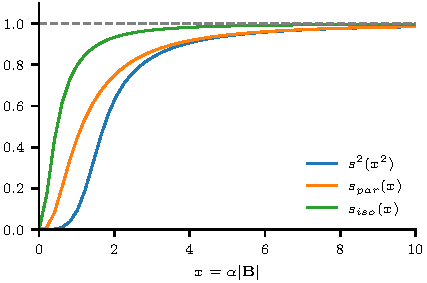
\includegraphics[width=0.5\linewidth]{alt_switching.pdf}
  \caption{The original switching function $s^2$ compared to the two possible interpolation function suggested by the Braginskii tensor. The interpolation rate of the functions are controlled by the parameters $a_0 = 36$ and $\alpha = 6$ which offer a direct comparison.}%
  \label{fig:alt_switching}
\end{figure}

The interpolation functions are easiest written using a form of $\eta_2(x)$ normalised against $\eta_0$,
\begin{equation}
  \label{eq:eta_function}
  \tilde{\eta}(x) = \eta_2(x)/\eta_0 = \frac{\tfrac{6}{5}x^2 + 2.23}{2.23 + 4.03 x^2 + x^4}.
\end{equation}
This allows us to define a new interpolation function based on the coefficient of the parallel part of the Braginskii tensor as
\begin{equation}
  \label{eq:alt_switching1}
s_{par}(x) = \frac{3+\tilde{\eta}(2x)-4\tilde{\eta}(x)}{3},
\end{equation}
and another based on the coefficient of the isotropic part,
\begin{equation}
  \label{eq:alt_switching2}
s_{iso}(x) = 1 - \tilde{\eta}(2x).
\end{equation}

Figure~\ref{fig:alt_switching} plots the two Braginskii interpolation functions and the switching function for parameter choices of $\alpha = 6$ and $a_0 = \alpha^2 = 36$. These parameter choices offer a direct comparison of the interpolation functions. The function $s_{par}$ shows the most similarity to the original switching function, particularly the shallow slope near $|\vec{B}| = 0$, in contrast to the steeper slope of $s_{iso}$. In order to understand the efficacy of each of these interpolation functions and how they compare to the full Braginskii model, more null point simulations were run and their results compared to those performed earlier. The computational efficiency of each model is also benchmarked using a short, low-resolution simulation.


\subsection{Calibrating the interpolation functions}

The parameter $a_0$ controls the effective size of the isotropic region by controlling the degree to which the viscosity is anisotropic for a given field strength. At $a = 30$, $s \approx 0.95$ and the viscosity may be considered anisotropic. If the viscosity should be considered anisotropic around $|\vec{B}| = B_0$, $a_0 = 30/B_0^2$. This may be linked to the degree to which a magnetic null is resolved, as illustrated in the proceeding example. 

In the numerical experiments performed in chapter~\ref{chp:null_point_khi}, the magnetic field strength increases linearly with distance from the null point and the grid separation is found to be $\Delta x \approx 0.014$. If we wish to consider the isotropic region extending over a radius of, say, ten grid points, the field at $x = 10 \Delta x$ is $|\vec{B}| = 0.14$, resulting in a calibrated $a_0 \approx 1500$. 


\section{Implementation of viscosity in Lare3D}

The two types of viscosity already present in the Lare3D code are shock and isotropic viscosities. Since shock viscosity is turned off for most numerical experiments presented in this thesis, I shall only detail the numerical implementation of isotropic viscosity, before discussing the implementations of the Braginskii and switching models.

\subsection{Review of the implementation of isotropic viscosity}

The isotropic viscous stress tensor is implemented in Lare3D as six 3D arrays, each storing the values for the six required components of a symmetric stress tensor. These are filled during the Lagrangian step using equation~\ref{eq:isotropic_viscous_tensor}, where the components of the strain rate tensor are calculated via equation~\ref{eq:rate_of_strain}. This stress tensor is used in the calculation of forces in the momentum equation and in the calculation of viscous heat contribution in the energy equation. This entire process is presented in detail below.

The strain rate tensor $\ten{W}$ is calculated in the code as \verb|s*|
\begin{verbatim}
sxx = (2.0_num * dvxdx - dvydy - dvzdz) * third
\end{verbatim}
for the diagonal elements \verb|sxx|, \verb|syy| and \verb|szz| and
\begin{verbatim}
sxy = dvxy * 0.5_num
\end{verbatim}
for the off-diagonal elements \verb|sxy|, \verb|sxz| and \verb|syz|. Since $\ten{W}$ is a symmetric tensor, only six components need to be calculated. The gradients of velocity, \verb|dv*|, are calculated using finite differences between appropriate velocity components, where the velocity is averaged over neighbouring grid points to ensure the resultant stress tensor is defined at the appropriate grid location. Note, the calculation of \verb|s*| in the code is a factor of a half smaller than the definition of $\ten{W}$ used in this thesis, equation~\ref{eq:rate_of_strain}. This is corrected for during the calculation of the viscous stress tensor, stored in the variable \verb|q*|, where a factor of two is included,
\begin{verbatim}
qxx(ix,iy,iz) = qxx(ix,iy,iz) + 2.0_num * sxx * rho(ix,iy,iz) * visc3
\end{verbatim}
and similarly for the other five components of the tensor. The multiplication by \verb|rho| at this point is cancelled out at a later stage.

The gradient of the tensor is used in the calculation of the forces in the momentum equation in the following way. The tensor values must be averaged to ensure the resultant gradient is correctly aligned with the velocity grid locations. Similar calculations are carried out for the other components of the stress tensor and force vector. This same code is used to include the anisotropic viscous stress tensors when they are enabled.
\begin{verbatim}
w1 = (qxx(ix ,iy ,iz ) + qxx(ix ,iyp,iz ) &
    + qxx(ix ,iy ,izp) + qxx(ix ,iyp,izp)) * 0.25_num
w2 = (qxx(ixp,iy ,iz ) + qxx(ixp,iyp,iz ) &
    + qxx(ixp,iy ,izp) + qxx(ixp,iyp,izp)) * 0.25_num
fx = fx + (w2 - w1) / dxc(ix)
\end{verbatim}

The viscous heat is calculated using
\begin{verbatim}
visc_heat(ix,iy,iz) = &
      qxy(ix,iy,iz) * dvxy  + qxz(ix,iy,iz) * dvxz &
    + qyz(ix,iy,iz) * dvyz  + qxx(ix,iy,iz) * dvxdx &
    + qyy(ix,iy,iz) * dvydy + qzz(ix,iy,iz) * dvzdz
\end{verbatim}
and, just as in the calculation of the forces above, this same code is used to calculate the viscous heat generated by the anisotropic viscous tensors when they are enabled.

\subsection{Implementation of the Braginskii tensor}

Since the contribution of a generic viscous stress tensor to the momentum and energy equations is already included in the numerical implementation of isotropic viscosity, the only new piece of code required to implement a new stress tensor is in the calculation of that stress tensor. The Braginskii tensor given by equation~\ref{eq:brag_new} is implemented in the following way and, when enabled, replaces the calculation of the isotropic viscous stress tensor. 

The four coefficients of the terms in equation~\ref{eq:brag_new} are calculated as
\begin{verbatim}
a = (3._num*visc3 + brag_visc1 - 4._num*brag_visc2)/MAX(2._num*mB2**2, none_zero)
b = (brag_visc1 - visc3)/(2._num*mB2)
c = (brag_visc2 - brag_visc1)/(mB2)
d = brag_visc1
\end{verbatim}
where \verb|visc3| is the variable holding the value of $\eta_0$, \verb|brag_visc1| and \verb|brag_visc2| hold the values of $\eta_1$ and $\eta_2$, calculated via equation~\ref{eq:perp_visc_coeff}, and \verb|mB2| holds the value of $|\vec{B}|^2$. This calculation is performed in the following way
\begin{verbatim}
xi2 = (brag_alpha**2) * mB2
brag_visc_coeff = visc3*(6._num/5._num*xi2 + 2.23_num)/(2.23_num + 4.03_num*xi2 + xi2**2)
\end{verbatim}
where \verb|brag_alpha| is the physics-dependent $\alpha = e \tau / m$ TODO explain this earlier.

The quantity $(\ten{W} \vec{B}) \cdot \vec{B})$ and the tensor components of $\vec{B} \otimes \vec{B}$ are calculated using the following snippet.
\begin{verbatim}
calc_wbdotb = 2._num*(&
  (bx*sxx + by*sxy + bz*sxz)*bx &
+ (bx*sxy + by*syy + bz*syz)*by &
+ (bx*sxz + by*syz + bz*szz)*bz)

btxx = bx**2
btyy = by**2
btzz = bz**2
btxy = bx*by
btxz = bx*bz
btyz = by*bz
\end{verbatim}

This allows the Braginskii stress tensor to be calculated using
\begin{verbatim}
bsxx = wbdotb*(a*btxx + b) + 2._num*d*sxx &
  + 4._num*c*(btxx*sxx + btxy*sxy + btxz*sxz)
\end{verbatim}
and similar for the diagonal \verb|bsxx|, \verb|bsyy| and \verb|bszz| components. The off-diagonal components are calculated using the following snippet.
\begin{verbatim}
bsxy = wbdotb*a*btxy + 2._num*d*sxy &
  + 2._num*c*(btxx* sxy + btxy* syy + btxz* syz &
            +  sxx*btxy +  sxy*btyy +  sxz*btyz)
\end{verbatim}

Finally, the contribution from the Braginskii stress tensor is added to the total stress tensor using 
\begin{verbatim}
qxx = qxx + rho*bsxx
\end{verbatim}
and similar for the other components. A later calculation in Lare3D requires that the Braginskii stress tensor is multiplied by \verb|rho|.

\subsection{Implementation of the switching model}

The numerical implementation of the switching model is similar to the implementation of the Braginskii model detailed previously, with the exception of the tensor itself which is calculated using
\begin{verbatim}
bsxx = visc3*((1.0_num-s2)*sxx*2.0_num + 1.5_num*s2/MAX(mB2**2, none_zero)*wbdotb*(btxx - mB2*third))
\end{verbatim}
and similar for the diagonal \verb|bsxx|, \verb|bsyy| and \verb|bszz| components. The off-diagonal components are calculated using the following snippet.
\begin{verbatim}
bsxy = visc3*((1.0_num-s2)*sxy*2.0_num + 1.5_num*s2/MAX(mB2**2, none_zero)*wbdotb*(btxy))
\end{verbatim}

The numerical implementation of the interpolation function itself is discussed in the following section.

\subsection{Spline representation of interpolation function}

Using a piecewise polynomial spline, $s$ was approximated using the following maple code.
\begin{verbatim}
with(Student[NumericalAnalysis]);
xy := [[0, 0], [0.5051, 0.02114], [1.54, 0.2023], [3.011, 0.508], [6.071, 0.7564], [12.97, 0.8854], [22.59, 0.9339], [29.41, 0.9492], [49, 0.97]];
p1 := CubicSpline(xy, independentvar = x);
expand(Interpolant(p1));
\end{verbatim}
The nodal value pairs contained within the variable \verb|xy| were calculated via the following maple code. The $x$ values were chosen to encourage a good fit.
\begin{verbatim}
kappa_erfi := a -> 1/2.0*(1 + 1/4*1/a) - 1/2*exp(2*a)/(sqrt(2*Pi*a)*erfi(sqrt(2*a)));
s2_erfi := a -> (1.0 + (-1)*3.0*kappa_erfi(a))^2;
\end{verbatim}

%0.0203207286957195 x+0.0843989591678155 x^3,x<0.5051
%0.0159559056317913-0.0744480634040214 x+0.187623821223007 x^2-0.0394206285197758 x^3,x<1.54
%-0.0887980204109068+0.129618026285783 x+0.0551133733724845 x^2-0.0107387134006150 x^3,x<3.011
%-0.498332905576744+0.537656769397807 x-0.0804026489164638 x^2+0.00426361387592081 x^3,x<6.071
%0.432999470914707+0.0774365207593949 x-0.00459631575250207 x^2+0.000101403742282107 x^3,x<12.97
%0.609014168122852+0.0367237920294194 x-0.00145732356052247 x^2+0.0000207305941973063 x^3,x<22.59
%0.852464153339503+0.00439311670189453 x-0.0000261294335846660 x^2-3.87808147946726 10^(-7) x^3,x<29.41
%0.816478868872687+0.00806383596073046 x-0.000150941377101699 x^2+0.00000102681208912720 x^3,otherwise

\todo{plot the spline}



\section{Application to stressed null point}

\label{sec:slow_null_point}

As a test of the switching model in a non-trivial topology, a series of simulations of magnetic null points subjected to twisting motions were carried out. Newtonian, full Braginskii and switching viscosities were used and the results compared.

\todo{describe ICs, BCs etc}

\subsection{Results}

\label{sec:slow_null_results}

The primary difference between isotropic and both anisotropic viscosity models is the magnitude and spatial distribution of the viscous heating. Isotropic viscosity overestimates the total heat generated by several orders of magnitude, when compared to either anisotropic model. The two anisotropic models differ in that the switching model vanishes where the Braginskii model does not, however it more clearly delineates the boundary between isotropic and anisotropic heating.

\subsubsection{Differences in viscous heating rates}

\begin{table}[t]
  \centering
  \caption{Total heat generated up to $t=10$ by each model of viscosity.}
  \label{tab:total_heating_slow_null}
  \begin{tabular}{ccccc}
Iso & Brag & Swi (von Mises) & Swi (par) & Swi (iso)\\
\midrule
$4.04 \times 10^{-3}$ & $5.25 \times 10^{-5}$ & $6.81 \times 10^{-5}$ & $7.80 \times 10^{-5}$ & $4.39 \times 10^{-5}$
\end{tabular}
\end{table}

Table~\ref{tab:total_heating_slow_null} shows the total heat generated by $t=10$ for each viscosity model. The isotropic model overestimates the viscous heating by approximately two orders of magnitude compared to any of the anisotropic models. The switching models all dissipate similar amounts of heat to the Braginskii model, indicating that these models are functioning correctly. The variance between each of the anisotropic models can be explained by considered how the isotropic and anisotropic parts of the tensors each contribute to the heating profile.

\begin{figure}[t]
    \centering
    \hfill
    \begin{subfigure}{0.32\textwidth}
      \includegraphics[width=1.0\linewidth]{iso_heating_iso_10.pdf}
      \caption{Isotropic}%
      \label{fig:iso_heating_iso_10}
    \end{subfigure}
    \hfill
    \begin{subfigure}{0.32\textwidth}
      \includegraphics[width=1.0\linewidth]{iso_heating_brag_10.pdf}
      \caption{Braginskii}%
      \label{fig:iso_heating_brag_10}
    \end{subfigure}
    \hfill
    \begin{subfigure}{0.32\textwidth}
      \includegraphics[width=1.0\linewidth]{iso_heating_switching_10.pdf}
      \caption{Switching (von Mises)}%
      \label{fig:iso_heating_switching_10}
    \end{subfigure}
    \begin{subfigure}{0.32\textwidth}
      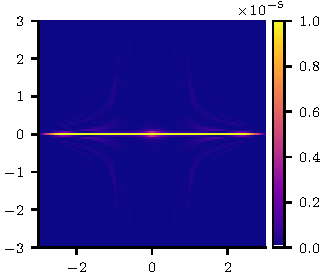
\includegraphics[width=1.0\linewidth]{iso_heating_switching2_10.pdf}
      \caption{Switching (par)}%
      \label{fig:iso_heating_switching2_10}
    \end{subfigure}
    \begin{subfigure}{0.32\textwidth}
      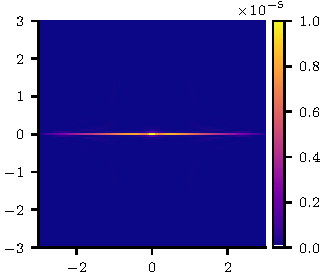
\includegraphics[width=1.0\linewidth]{iso_heating_switching3_10.pdf}
      \caption{Switching (iso)}%
      \label{fig:iso_heating_switching3_10}
    \end{subfigure}

    \caption{A comparison of the isotropic heating generated by the isotropic, full Braginskii and switching models at time $t=10$, sliced through $y=0$. Note the peak colour of the isotropic plot is an order of magnitude greater than that of the anisotropic models. The isotropic model overestimates local heating by an order of magnitude and heats more extensively throughout the null. The heating distribution generated by the isotropic switching model best matches that of the Braginskii model. Due to the numerical implementation of the von Mises switching function, some isotropic heating far from the null is neglected.}
\label{fig:isotropic_heating}%
\end{figure}

Figure~\ref{fig:isotropic_heating} shows the isotropic heating rate at time $t=10$ for each viscosity model. Isotropic viscosity heats at a generally greater rate than the anisotropic models, and the heating is distributed more extensively throughout the null. The erroneously sharp boundary where isotropic viscosity turns off in the von Mises switching model can be seen in figure~\ref{fig:iso_heating_switching_10}. The heating generated by the two Braginskii-inspired models show most similarity to that of the Braginskii model, with the isotropic-based switching model showing a nearly identical heating profile. This is to be expected since the coefficients of the isotropic contributions to the Braginskii and isotropic-based switching tensors are identical. The relative magnitude of the isotropic heating contributions for each anisotropic model reflects the total heat generated in table~\ref{tab:total_heating_slow_null}.

\begin{figure}[t]
    \hfill
    \begin{subfigure}{0.49\textwidth}
      \includegraphics[width=1.0\linewidth]{aniso_heating_brag_10.pdf}
      \caption{Braginskii}%
      \label{fig:aniso_heating_brag_10}
    \end{subfigure}
    \hfill
    \begin{subfigure}{0.49\textwidth}
      \includegraphics[width=1.0\linewidth]{aniso_heating_switching_10.pdf}
      \caption{Switching (von Mises)}%
      \label{fig:aniso_heating_switching_10}
    \end{subfigure}
    \hfill
    \begin{subfigure}{0.49\textwidth}
      \includegraphics[width=1.0\linewidth]{aniso_heating_switching2_10.pdf}
      \caption{Switching (par)}%
      \label{fig:aniso_heating_switching2_10}
    \end{subfigure}
    \hfill
    \begin{subfigure}{0.49\textwidth}
      \includegraphics[width=1.0\linewidth]{aniso_heating_switching3_10.pdf}
      \caption{Switching (iso)}%
      \label{fig:aniso_heating_switching3_10}
    \end{subfigure}
    \caption{A comparison of the anisotropic heating generated by the full Braginskii and switching models at time $t=10$. Close to the fan plane the Braginskii model shows notably greater anisotropic heating than any of the switching models. The switching models all appear similar though with minor differences near the null point.}
\label{fig:anisotropic_heating}%
\end{figure}

Figure~\ref{fig:anisotropic_heating} shows the contributions to viscous heating from the anisotropic parts of the Braginskii and switching tensors. The anisotropic heating generated by the Braginskii tensor is dominated by the perpendicular contribution near the fan plane. This reveals the potential issue with artificially increasing $\alpha$, that alongside increasing the size of the isotropic region, the extent of the perpendicular contributions are similarly enhanced. This may be a desirable feature of a model of anisotropic viscosity, however the switching models avoid this effect completely. In this way, the switching models provide a useful compromise.

\subsubsection{The effect of resolution on the size of the isotropic region}

\begin{table}[t]
  \centering
  \caption{Total heat generated up to $t=10$ by each model of viscosity for resolutions of $N=100$ and $500$.}
  \label{tab:slow_null_results_resolution}
  \begin{tabular}{c|cccc}
Model &  Brag & Swi (von Mises) & Swi (par) & Swi (iso)\\
\midrule
$N=100$ &  $5.74 \times 10^{-5}$ & $7.13 \times 10^{-5}$ & $8.39 \times 10^{-5}$ & $4.66 \times 10^{-5}$\\
$N=500$   & $5.25 \times 10^{-5}$ & $6.81 \times 10^{-5}$ & $7.80 \times 10^{-5}$ & $4.39 \times 10^{-5}$  \end{tabular}
\end{table}

\begin{figure}[t]
    \hfill
    \begin{subfigure}{0.49\textwidth}
      \centering
      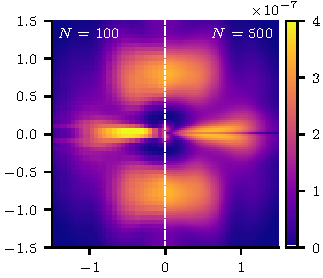
\includegraphics[width=1.0\linewidth]{diff_brag_resolution.pdf}
      \caption{Braginskii}%
      \label{fig:diff_brag_resolution}
    \end{subfigure}
    \hfill
    \begin{subfigure}{0.49\textwidth}
      \includegraphics[width=1.0\linewidth]{diff_switching_resolution.pdf}
      \caption{Switching (von Mises)}%
      \label{fig:diff_switching_resolution}
    \end{subfigure}
    \hfill
    \begin{subfigure}{0.49\textwidth}
      \includegraphics[width=1.0\linewidth]{diff_switching2_resolution.pdf}
      \caption{Switching (par)}%
      \label{fig:diff_switching2_resolution}
    \end{subfigure}
    \hfill
    \begin{subfigure}{0.49\textwidth}
      \includegraphics[width=1.0\linewidth]{diff_switching3_resolution.pdf}
      \caption{Switching (iso)}%
      \label{fig:diff_switching3_resolution}
    \end{subfigure}

    \caption{A comparison between the anisotropic heating rates produced by the Braginskii and switching models at resolutions of $100$ (left of each plot) and $500$ (right of each plot) grid points per dimension. Both plots are slices through $x=0$ at $t=5$. When the null point is less resolved (left half of both figures) Braginskii viscosity erroneously permits anisotropic heating at the null. At higher resolutions (left half of both figures) the null is better resolved and much less anisotropic viscous heating is found at the null. All switching models avoid this issue.}
\label{fig:anisotropy_bleeding}%
\end{figure}

Identical simulations were run to those described in~\ref{sec:slow_null_results} but with the resolution reduced to $N=100$ per dimension. This allows a clear demonstration of the effect of poor resolution on the accurate estimate of isotropic heating, even when $\alpha$ is artificially increased in the Braginskii model. While table~\ref{tab:slow_null_results_resolution} shows the global estimate of total viscous heat is relatively accurate at a low resolution, figure~\ref{fig:anisotropic_heating} shows that the spatial distribution of the heating rate is less so.

Figure~\ref{fig:anisotropy_bleeding} shows the heating rate produced by the anisotropic parts of the Braginskii and switching models and reveals the primary issue with the Braginskii model. When the resolution is too low to properly resolve the region around the null point, the Braginskii model erroneously heats anisotropically. This is primarily due to the artificially increased $\alpha$ enhancing the perpendicular components near the null point. This issue is mitigated by the switching models, all of which remove the perpendicular components of the Braginskii tensor. At the higher resolution of $N=500$ the von Mises switching model does remove a small portion of realistic anisotropic heating near the null. Both Braginskii-based switching models appear to approximate the Braginskii tensor more accurately. Away from the null the switching models give adequately similar results to the Braginskii model.

\section{Model efficiency}

In order to evaluate the real efficiency of each model of viscosity, a set of benchmark tests were run with the same physical setup as that of the test simulations found in section~\ref{sec:slow_null_point}, although changing the initial or boundary conditions should not affect the results. The resolution is set to $N=100$, all output is disabled, only one CPU core is used, and the simulations run for only $100$ timesteps. This number of timesteps allows the main loop of the simulation to run for a longer time than the overhead required to start and end the simulation, giving a more accurate estimate of the running time. The combination of the resolution and the number of timesteps results in the viscosity routines running $10^{8}$ times per simulation. The time is calculated via the linux \verb|time| command which reports millisecond accuracy. Due to other software running on the same machine, the total time can vary. To measure a more accurate running time, the test for each model is repeated $25$ times and the results averaged. The machine used to run these tests is a Dell all-in-one with a 4 core, Intel i7-6700 CPU running at 3.4 GHz and 16 GB of RAM. 

\todo{figure}

%Figure~\todo{fig} shows the average measured runtime for each model. Since the isotropic model requires only the calculation of the rate of strain tensor, it is the quickest. The Braginskii model, being the most complex, requires many additional calculations to be carried out and this is reflected in its relatively poor runtime. The switching models show similar efficiencies, worse than the isotropic model but significantly better than the Braginskii model, as expected from considering the number of required calculations. The differences between the runtimes of the different interpolation functions are slight, although the von Mises implementation appears moderately faster. 

\section{Conclusion}

This chapter details the development of the switching model, a new model of anisotropic viscosity specifically designed for use in numerical simulations of the solar corona. The model improves on the Braginskii model by artificially enlarging the easily under-resolved isotropic region surrounding magnetic null points. The switching model does this by exposing a tunable interpolation function which measures the degree of anisotropy (dependent on the local magnetic field strength) and interpolates between isotropic and fully field-aligned viscosity. Three candidate interpolation functions are presented and their accuracy, efficacy and computational efficiency compared. The switching model is found to be computationally more efficient than the Braginskii model and offers an acceptable approximation to it. 
